\subsection{The first existence theorem}

DEFINITION 1. Let A, A' be two rings and h: A → A' a ring homomorphism. An ideal a' of A' is said to lie above an ideal a of A if \iffalse h\^{}\{-1\}(a')\fi\(a = h^{-1}(a')\).

To say that a prime ideal \(\mathfrak{p}'\) of \(\mathbf{A}'\) lies above an ideal \(\mathfrak{p}\) of \(\mathbf{A}\) therefore means that \(\mathfrak{p}\) is the image of \(\mathfrak{p}'\) under the continuous mapping \(^a h\) : \(\operatorname{Spec}(\mathbf{A}') \to \operatorname{Spec}(\mathbf{A})\) associated with \(h\) (Chapter II, § 4, no. 3).

Note that for there to exist an ideal of \(\mathbf{A}'\) lying above the ideal (0) of \(\mathbf{A}\) , it is necessary and sufficient that \(h: \mathbf{A} \to \mathbf{A}'\) be injective.

Let \(\mathfrak{a}\) be an ideal of \(\mathbf{A}\) ; by taking quotients the homomorphism \(h\) gives a homomorphism \(h_1: \mathbf{A} / \mathfrak{a} \to \mathbf{A}' / \mathfrak{a}'\) ; to say that \(\mathfrak{a}'\) is an ideal of \(\mathbf{A}'\) lying above \(\mathfrak{a}\) is equivalent to saying that \(\mathfrak{a}\mathbf{A}' \subset \mathfrak{a}'\) and that \(\mathfrak{a}' / \mathfrak{a}\mathbf{A}'\) is an ideal of \(\mathbf{A}' / \mathfrak{a}\mathbf{A}'\) lying above (0).

LEMMA 1. Let \(h: \mathbf{A} \to \mathbf{A}'\) be a ring homomorphism, \(\mathbf{S}\) a multiplicative subset of \(\mathbf{A}\) , \(i = i_{\mathbf{A}}^{\mathbf{S}}: \mathbf{A} \to \mathbf{S}^{-1}\mathbf{A}\) , \(i' = i_{\mathbf{A}'}^{h(\mathbf{S})}: \mathbf{A}' \to \mathbf{S}^{-1}\mathbf{A}' = (h(\mathbf{S}))^{-1}\mathbf{A}'\) the canonical homomorphisms and \(h_1 = \mathbf{S}^{-1}h: \mathbf{S}^{-1}\mathbf{A} \to \mathbf{S}^{-1}\mathbf{A}'\) , so that there is a commutative diagram

\pandocbounded{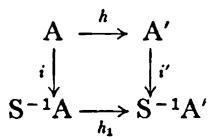
\includegraphics[keepaspectratio]{images/part002_a0a90333.jpg}}

Let \(\mathfrak{p}\) be a prime ideal of \(\mathbf{A}\) such that \(\mathfrak{p} \cap \mathbf{S} = \varnothing\) . Then \(\mathfrak{a}' \mapsto \mathbf{S}^{-1}\mathfrak{a}'\) is a surjective mapping of the set \(\mathcal{F}\) of ideals of \(\mathbf{A}'\) lying above \(\mathfrak{p}\) onto the set \(\mathcal{F}_1\) of ideals of \(\mathbf{S}^{-1}\mathbf{A}'\) lying above \(\mathbf{S}^{-1}\mathfrak{p}\) and the mapping \(\mathfrak{a}_1' \mapsto i'^{-1}(\mathfrak{a}_1')\) is a bijection of \(\mathcal{F}_1\) onto the set of ideals belonging to \(\mathcal{F}\) and is saturated with respect to \(h(S)\) ; in particular \(\mathfrak{p}' \mapsto \mathbf{S}^{-1}\mathfrak{p}'\) is a bijection of the set of prime ideals of \(\mathbf{A}'\) lying above \(\mathfrak{p}\) onto the set of prime ideals of \(\mathbf{S}^{-1}\mathbf{A}'\) lying above \(\mathbf{S}^{-1}\mathfrak{p}\) .

We know that \(\mathbf{S}^{-1}\mathfrak{p}\) is a prime ideal of \(\mathbf{S}^{-1}\mathbf{A}\) and that \(i^{-1}(\mathbf{S}^{-1}\mathfrak{p}) = \mathfrak{p}\) (Chapter II, § 2, no. 5, Proposition 11); if there exists an ideal \(\mathfrak{b}'\) of \(\mathbf{S}^{-1}\mathbf{A}'\) lying above \(\mathbf{S}^{-1}\mathfrak{p}\) , then \(h(i'^{-1}(\mathfrak{b}')) = i^{-1}(h_1(\mathfrak{b}')) = \mathfrak{p}\) ; as \(\mathbf{S}^{-1}.i'^{-1}(\mathfrak{b}') = \mathfrak{b}'\) (loc. cit.), this already shows that the image of \(\mathcal{F}\) under the mapping \(\mathfrak{a}'\mapsto\mathrm{S}^{-1}\mathfrak{a}'\) contains \(\mathcal{F}_{1}\) . On the other hand, if \(\mathfrak{a}'\in\mathcal{F}\) , \(a\in\mathbf{A}\) and \(s\in\mathbf{S}\) , there are the following equivalences

\[
\begin{array}{l} h _ {1} (a / s) \in \mathrm{S} ^ {- 1} \mathfrak {a} ^ {\prime} \Leftrightarrow h (a) / h (s) \in \mathrm{S} ^ {- 1} \mathfrak {a} ^ {\prime} \\ \Leftrightarrow \text { there   exists } t \in \mathrm{S} \text { such   that } h (t) h (a) \in \mathfrak {a} ^ {\prime} \\ \Leftrightarrow \text { there   exists } t \in \mathrm{S} \text { such   that } t a \in \mathfrak {p} \\ \Leftrightarrow a / s \in \mathrm{S} ^ {- 1} \mathfrak {p}. \end{array}
\]

Hence \(h_1^{-1}(\mathbf{S}^{-1}\mathfrak{a}') = \mathbf{S}^{-1}\mathfrak{p}\) , which completes the proof that the image of \(\mathcal{F}\) under the mapping \(\mathfrak{a}' \mapsto \mathbf{S}^{-1}\mathfrak{a}'\) is equal to \(\mathcal{F}_1\) ; the other assertions follow from Chapter II, § 2, no. 5, Proposition 11.

PROPOSITION 1. Let \(h: \mathbf{A} \to \mathbf{A}'\) be a ring homomorphism such that \(\mathbf{A}'\) is integral over \(\mathbf{A}\) , \(\mathfrak{p}'\) a prime ideal of \(\mathbf{A}'\) and \(\mathfrak{p} = h^{-1}(\mathfrak{p}')\) . For \(\mathfrak{p}\) to be maximal, it is necessary and sufficient that \(\mathfrak{p}'\) be so.

Let us write \(\mathrm{B} = \mathrm{A} / \mathfrak{p}\) , \(\mathrm{B}' = \mathrm{A}' / \mathfrak{p}'\) and let \(h_1 \colon \mathrm{B} \to \mathrm{B}'\) be the homomorphism derived from \(h\) by taking quotients; \(\mathrm{B}\) and \(\mathrm{B}'\) are integral domains and \(\mathrm{B}'\) is integral over \(\mathrm{B}\) (§ 1, no. 1, Proposition 2). To say that \(\mathfrak{p}\) (resp. \(\mathfrak{p}'\) ) is maximal means that \(\mathrm{B}\) (resp. \(\mathrm{B}'\) ) is a field. The proposition then follows from the following lemma:

LEMMA 2. Let B be an integral domain and A a subring of B such that B is integral over A. For B to be a field, it is necessary and sufficient that A be a field.

If A is a field, then, for all \(y \neq 0\) in B, A[y] is by hypothesis ( \(\S 1\) , Theorem 1) a finitely generated A-module; as A[y] is an integral domain, it is a field (Algebra, Chapter V, \(\S 2\) , no. 1, Proposition 1) and a fortiori y is invertible in B and hence B is a field. Conversely, suppose that B is a field and let \(z \neq 0\) in A; as \(z^{-1} \in B\) , \(z^{-1}\) is integral over A, in other words there is an equation of integral dependence

\[
z ^ {- n} + a _ {1} z ^ {- (n - 1)} + \dots + a _ {n} = 0
\]

where the \(a_{i} \in \mathbf{A}\) ; now this relation shows that

\[
- z ^ {- 1} = a _ {1} + a _ {2} z + \dots + a _ {n} z ^ {n - 1} \in A,
\]

hence A is certainly a field.

COROLLARY 1. Let \(h: \mathbf{A} \to \mathbf{A}'\) be a ring homomorphism such that \(\mathbf{A}'\) is integral over \(\mathbf{A}\) , \(\mathfrak{p}\) a prime ideal of \(\mathbf{A}\) and \(\mathfrak{p}'\) and \(\mathfrak{a}'\) two ideals of \(\mathbf{A}'\) lying above \(\mathfrak{p}\) such that \(\mathfrak{p}' \subset \mathfrak{a}'\) . If \(\mathfrak{p}'\) is prime, then \(\mathfrak{a}' = \mathfrak{p}'\) .

Let us write \(S = A - p\) ; then \(S^{-1}A'\) is integral over \(S^{-1}A\) (§ 1, no. 5, Proposition

16), \(S^{-1}p\) is a maximal ideal of \(S^{-1}A\) (Chapter II, §2, no. 5, Proposition 11), \(S^{-1}a'\) and \(S^{-1}p'\) are ideals of \(S^{-1}A'\) lying above \(S^{-1}p\) (Lemma 1) and \(S^{-1}a' \supseteq S^{-1}p'\) . As \(S^{-1}p'\) is prime, it is maximal by Proposition 1 and hence \(S^{-1}p' = S^{-1}a'\) ; therefore \(a'\) is contained in the saturation of \(p'\) with respect to \(h(S)\) , which is equal to \(p'\) (Chapter II, §2, no. 5, Proposition 11).

COROLLARY 2. Let A' be an integral domain, A a subring of A' such that A' is integral over A and f a homomorphism from A' to a ring B. If the restriction of f to A is injective, f is injective.

If \(a'\) is the kernel of f, the hypothesis means that \(a' \cap A = (0)\) ; as \(A'\) is an integral domain, Corollary 1 may be applied taking p and \(p'\) to be the ideal (0) of A and the ideal (0) of \(A'\) respectively, whence \(a' = (0)\) .

COROLLARY 3. Let \(h: \mathbf{A} \to \mathbf{A}'\) be a ring homomorphism such that \(\mathbf{A}'\) is integral over \(\mathbf{A}\) and \(\mathfrak{m}\) a maximal ideal of \(\mathbf{A}\) and suppose that there are in \(\mathbf{A}'\) only a finite number of distinct maximal ideals \(\mathfrak{m}_j' (1 \leqslant j \leqslant n)\) lying above \(\mathfrak{m}\) . Let \(\mathfrak{q}_j'\) be the saturation of \(\mathfrak{mA}'\) with respect to \(\mathfrak{m}_j'\) (Chapter II, § 2, no. 4). Then:

\begin{enumerate}
\def\labelenumi{(\roman{enumi})}
\item
  In the ring \(\mathbf{A}' / \mathfrak{q}_j'\) the divisors of zero are the elements of \(\mathfrak{m}_j' / \mathfrak{q}_j'\) and they are nilpotent ( \(1 \leqslant j \leqslant n\) ).
\item
  \(mA' = \bigcap_{j} q_{j}' = \prod_{j} q_{j}'\) .
\item
  The canonical homomorphism \(\mathbf{A}' / \mathfrak{m}\mathbf{A}' \to \prod_j (\mathbf{A}' / \mathfrak{q}_j')\) is bijective.
\end{enumerate}

For a prime ideal of A' to contain mA', it is necessary and sufficient that its inverse image under h contain m and hence that it lie above m, since m is maximal in A; the \(m_{j}'\) are therefore the only prime ideals of A' containing mA' (Proposition 1) and therefore \(r' = \bigcap_{j} m_{j}'\) is the radical of mA' (Chapter II, §2, no. 6, Corollary 1 to Proposition 13). By definition of \(q_{j}'\) , the class mod. \(q_{j}'\) of an element of \(\mathbf{A}' - \mathfrak{m}_{j}'\) is not a divisor of 0 in \(A'/q_{j}'\); on the other hand, as the \(m_{j}'\) are distinct maximal ideals, for every index j there exists an element \(a_{j}'\) belonging to \(\bigcap_{i \neq j} m_{i}'\) and not to \(m_{j}'\) (Chapter II, §1, no. 1, Proposition 4); then, for all \(x \in m_{j}'\) , \(a_{j}'x \in r'\) , hence the class mod. \(q_{j}'\) of \(a_{j}'x\) is nilpotent and, as that of \(a_{j}'\) is not a divisor of 0, we conclude that the class of x is nilpotent; in other words \(m_{j}'\) is the radical of \(q_{j}'\) , which proves (i). It follows that the \(q_{j}'\) are relatively prime in pairs (Chapter II, §1, no. 1, Proposition 3); (iii) will therefore be a consequence of (ii), taking account of Chapter II, §1, no. 2, Proposition 5. To establish (ii), we note that in the ring A'/mA' the \(m_{j}'/mA'\) are the only maximal ideals and \(q_{j}'/mA'\) is the saturation of (0) with respect to \(m_{j}'/mA'\) (Chapter II, §2, no. 4); we may therefore restrict our attention to the case mA' = (0); the assertion of (ii) then follows from Chapter II, §3, no. 3, Corollary 2 to Theorem 1.

Remark (1) If \(\mathbf{A}'\) is Noetherian, it follows from (i) and (ii) that \((\mathfrak{q}_j')_{1 \leqslant j \leqslant n}\) is the unique primary decomposition of \(\mathfrak{mA}'\) (Chapter IV, § 2, no. 3).

THEOREM 1. Let \(h: \mathbf{A} \to \mathbf{A}'\) be an injective ring homomorphism such that \(\mathbf{A}'\) is integral over \(\mathbf{A}\) and \(\mathfrak{p}\) a prime ideal of \(\mathbf{A}\) . There exists a prime ideal \(\mathfrak{p}'\) of \(\mathbf{A}'\) lying above \(\mathfrak{p}\) .

Suppose first that A is a local ring and p the maximal ideal of A; then, for every maximal ideal \(m'\) of \(A'\) , \(\bar{h}^{-1}(m')\) is a maximal ideal of A (Proposition 1) and hence equal to p, which proves the theorem in this case (since \(A'\) contains A by hypothesis and is therefore not reduced to 0). In the general case, let us write \(S = A - p\) ; then \(S^{-1}A\) is a local ring whose maximal ideal is \(S^{-1}p\) (Chapter II, §2, no. 5, Proposition 11), \(S^{-1}h: S^{-1}A \to S^{-1}A'\) is injective (Chapter II, §2, no. 4, Theorem 1) and \(S^{-1}A'\) is integral over \(S^{-1}A\) (§1, no. 5, Proposition 16); then there exists a prime ideal \(q'\) of \(S^{-1}A'\) lying above \(S^{-1}p\) and we know that \(q' = S^{-1}p'\) , where \(p'\) is a prime ideal of \(A'\) lying above p (Lemma 1).

If \(h: \mathbf{A} \to \mathbf{A}'\) is not injective, Theorem 1 is no longer necessarily true, as the example of the homomorphism \(\mathbf{Z} \to \mathbf{Z}/n\mathbf{Z}\) ( \(n > 1\) ) shows. However Theorem 1 can be applied to the canonical injection \(h(\mathbf{A}) \to \mathbf{A}'\) ; in other words, the statement of Theorem 1 is true for prime ideals \(\mathfrak{p}\) containing \(\operatorname{Ker}(h)\) .

COROLLARY 1. With the hypotheses and notation of Theorem 1, \(h^{-1}(pA') = p\) .

\(\mathfrak{pA}' \subset \mathfrak{p}'\) and \(\overline{h}(\mathfrak{p}') = \mathfrak{p}\) .

COROLLARY 2. Let \(h: \mathbf{A} \to \mathbf{A}'\) be a ring homomorphism such that \(\mathbf{A}'\) is integral over \(\mathbf{A}\) , \(\mathfrak{a}\) and \(\mathfrak{p}\) two ideals of \(\mathbf{A}\) such that \(\mathfrak{a} \subset \mathfrak{p}\) and \(\mathfrak{a}'\) an ideal of \(\mathbf{A}'\) lying above \(\mathfrak{a}\) . Suppose that \(\mathfrak{p}\) is prime. Then there exists a prime ideal \(\mathfrak{p}'\) of \(\mathbf{A}'\) lying above \(\mathfrak{p}\) and containing \(\mathfrak{a}'\) .

If \(h_1 \colon \mathbf{A} / \mathfrak{a} \to \mathbf{A}' / \mathfrak{a}'\) is the homomorphism derived from \(h\) by taking quotients, \(h_1\) is injective by hypothesis and \(\mathbf{A}' / \mathfrak{a}'\) is integral over \(\mathbf{A} / \mathfrak{a}\) (§ 1, no. 1, Proposition 2); then there exists a prime ideal \(\mathfrak{p}' / \mathfrak{a}'\) of \(\mathbf{A}' / \mathfrak{a}'\) ( \(\mathfrak{p}'\) prime in \(\mathbf{A}'\) ) lying above \(\mathfrak{p} / \mathfrak{a}\) (Theorem 1) and \(\mathfrak{p}'\) is the required ideal.

COROLLARY 3. Let A be a ring and A' a ring containing A and integral over A. If R' is the Jacobson radical of A', R' ∩ A is the Jacobson radical of A.

Let \(\mathfrak{R}\) be the Jacobson radical of A. For every maximal ideal \(\mathfrak{m}'\) of \(\mathbf{A}'\) , \(\mathfrak{m}' \cap \mathbf{A}\) is a maximal ideal of A (Proposition 1), hence \(\mathfrak{R} \subset \mathfrak{m}' \cap \mathbf{A}\) and therefore \(\mathfrak{R} \subset \mathfrak{R}' \cap \mathbf{A}\) (Algebra, Chapter VIII, § 5, no. 3, Definition 3). Conversely, let \(x \in \mathfrak{R}' \cap \mathbf{A}\) ; for every maximal ideal \(\mathfrak{m}\) of A, there exists a prime ideal of \(\mathbf{A}'\) lying above \(\mathfrak{m}\) (Theorem 1) and this ideal \(\mathfrak{m}'\) is necessarily maximal (Proposition 1), hence \(x \in \mathfrak{m}' \cap \mathbf{A} = \mathfrak{m}\) and therefore \(x \in \mathfrak{R}\) .

COROLLARY 4. Let A be a ring, A' a ring containing A and integral over A and f a homomorphism from A to an algebraically closed field L. Then f can be extended to a homomorphism from A' to L.

Let p be the kernel of f, which is a prime ideal since \(f(\mathbf{A}) \subset \mathbf{L}\) is an integral domain; let \(p'\) be a prime ideal of \(A'\) lying above p (Theorem 1). Then A/p is canonically identified with a subring of \(A'/p'\) and \(A'/p'\) is integral over A/p (§ 1, no. 1, Proposition 2). The homomorphism f defines, by taking the quotient, an isomorphism of A/p onto the subring \(f(\mathbf{A})\) of L, which can be extended to an isomorphism g of the field of fractions K of A/p onto a subfield of L. As the field of fractions \(K'\) of \(A'/p'\) is algebraic over K, g can be extended to an isomorphism \(g'\) of \(K'\) onto a subfield of L (Algebra, Chapter V, § 4, no. 2, Corollary to Theorem 1); if \(\pi': A' \to A'/p'\) is the canonical homomorphism, \(g' \circ \pi'\) is a homomorphism from \(A'\) to L extending f.

Remark (2). Let \(h \colon \mathbf{A} \to \mathbf{A}'\) be a ring homomorphism such that \(\mathbf{A}'\) is integral over \(\mathbf{A}\) ; then the associated continuous mapping \(^a h \colon \operatorname{Spec}(\mathbf{A}') \to \operatorname{Spec}(\mathbf{A})\) is closed. For every ideal \(\mathfrak{a}'\) of \(\mathbf{A}'\) , \(\mathbf{A}' / \mathfrak{a}'\) is integral over \(\mathbf{A}'\) , hence also over \(\mathbf{A}\) (§ 1, no. 1, Proposition 6) and \(\operatorname{Spec}(\mathbf{A}' / \mathfrak{a}')\) is identified with a closed subspace \(\mathbf{V}(\mathfrak{a}')\) of \(\operatorname{Spec}(\mathbf{A}')\) ; to show that \(^a h\) is closed, we see then (replacing \(\mathbf{A}'\) by \(\mathbf{A}' / \mathfrak{a}'\) ) that it is sufficient to prove that the image of \(\operatorname{Spec}(\mathbf{A}')\) under \(^a h\) is a closed subset of \(\operatorname{Spec}(\mathbf{A})\) ; now it follows from Theorem 1 that this image is just the set of prime ideals of \(\mathbf{A}\) containing the ideal \(\operatorname{Ker}(h)\) and this set is closed by definition of the topology on \(\operatorname{Spec}(\mathbf{A})\) .

PROPOSITION 2. Let \(h: \mathbf{A} \to \mathbf{A}'\) be a ring homomorphism such that \(\mathbf{A}'\) is integral over \(\mathbf{A}\) , \(\mathfrak{p}\) a prime ideal of \(\mathbf{A}\) , \(S = A - \mathfrak{p}\) , \((\mathfrak{p}_i')_{i \in I}\) the family of all the prime ideals of \(\mathbf{A}'\) lying above \(\mathfrak{p}\) and \(S' = \bigcap_{i \in I} (\mathbf{A}' - \mathfrak{p}_i')\) ; then \(S^{-1}A' = S'^{-1}A'\) .

In fact, by definition \(h(\mathbf{S}) \subset \mathbf{S}'\) and, as

\[
h (\mathbf {S}) ^ {- 1} \mathbf {A} ^ {\prime} = \mathbf {S} ^ {- 1} \mathbf {A} ^ {\prime},
\]

it suffices to prove, by virtue of Chapter II, § 2, no. 3, Proposition 8, that, if a prime ideal \(\mathfrak{q}'\) of \(\mathbf{A}'\) does not meet \(h(\mathbf{S})\) , it does not meet \(\mathbf{S}'\) either. Now, suppose that \(\mathfrak{q}' \cap h(\mathbf{S}) = \varnothing\) and let \(\mathfrak{q} = \bar{h}^{-1}(\mathfrak{q}')\) ; then \(\mathfrak{q} \cap \mathbf{S} = \varnothing\) , in other words \(\mathfrak{q} \subset \mathfrak{p}\) . As \(\mathfrak{q}'\) lies above \(\mathfrak{q}\) by definition, it follows from Corollary 2 to Proposition 1 that there is an index \(\iota\) such that \(\mathfrak{q}' \subset \mathfrak{p}_i'\) and hence \(\mathfrak{q}' \cap \mathbf{S}' = \varnothing\) , which completes the proof.

PROPOSITION 3. Let \(h: \mathbf{A} \to \mathbf{A}'\) be a ring homomorphism such that \(\mathbf{A}'\) is a finitely generated A-module; then, for every prime ideal \(\mathfrak{p}\) of \(\mathbf{A}\) , the set of prime ideals of \(\mathbf{A}'\) lying above \(\mathfrak{p}\) is finite.

Let \(S = A - p\) ; by Lemma 1 we may replace \(A\) by \(S^{-1}A\) , \(A'\) by \(S^{-1}A'\) (which is a finitely generated \(S^{-1}A\) -module) and \(p\) by \(S^{-1}p\) ; in other words, we may assume that \(A\) is a local ring and \(p\) is its maximal ideal. Then (by the remark made at the beginning of this no.) A may be replaced by \(A/p\) , \(A'\) by \(A'/pA'\) and \(p\) by (0), for \(A'/pA' = (A/p) \otimes_A A'\) is a finitely generated \((A/p)\) -module. Thus we have finally reduced the problem to proving the proposition when \(A\) is a field and \(p = (0)\) ; \(A'\) is then an \(A\) -algebra of finite rank and therefore Artinian and we know that in such an algebra there is only a finite number of prime ideals (Chapter IV, § 2, no. 5, Proposition 9).

